\documentclass{article}
\usepackage{graphicx}
\usepackage{wrapfig}
\usepackage{subcaption}
\usepackage[margin=1in]{geometry}
\usepackage{amsmath,amssymb} 
\usepackage{siunitx}
\usepackage{booktabs}
\usepackage[export]{adjustbox}
\newcommand{\angstrom}{\textup{\AA}}
\newcommand{\colormap}{jet}  % colorbar to use
\usepackage{cleveref}
\usepackage{booktabs}
\usepackage{gensymb}
\usepackage{float}
\usepackage{hyperref}
\title{Simulated Structure Factors}
\author{Benjamin J. Coscia}
\begin{document}
  \graphicspath{{./figures/}}
  \maketitle

  \section{Calculation of the structure factor}

  The structure factor, S($\mathbf{q}$), relates the observed intensity per
  atom to that observed by a single scattering unit. Incident plane waves falling
  on a material have a wave vector, $K_i$, whose length is
  $\dfrac{2\pi}{\lambda}$, where $\lambda$ is the wavelength. The diffracted wave
  vector, $K_f$, has the same length as $K_i$ if the diffraction process is 
  elastic. We will assume elasticity going forward. The scattering vector, $\mathbf{q}$,
  is defined as $K_f - K_i$. Since $K_f$ and $K_i$ are the same length, the scattering
  vector must lie on the surface of a sphere of radius $\dfrac{2\pi}{\lambda}$. This
  sphere is called the Ewald Sphere and diffraction will only occur for reciprocal
  lattice points that lie on its surface. 

  The amplitude and phase of the scattered waves is the vector sum of all scattered 
  waves from all atoms:

  \begin{equation}\label{eq:dft}
  \Psi_s(\mathbf{q}) = \sum_{j=1}^{N}f_je^{-i\mathbf{q}\boldsymbol{\cdot}\mathbf{R_j}}
  \end{equation}

  where $f_j$ is the atomic form factor of atom $j$ and $\mathbf{R_j}$ is the position of
  the atom in real space. Note that Equation 1 %\eqref{eq:dft} %equation reference not working for some reason
  is the definition of the discrete fourier transform.

  The scattered intensity is obtained by multiplying Equation 1%\eqref{eq:dft} 
  by its complex conjugate:
  \begin{equation}\label{eqn:conjugate}
  I(\mathbf{q}) = \Psi_s(\mathbf{q})\cdot\overline{\Psi_s}(\mathbf{q}) = \sum_{j=1}^{N}f_je^{-i\mathbf{q}\boldsymbol{\cdot}\mathbf{R_j}} \times \sum_{k=1}^{N}f_ke^{-i\mathbf{q}\boldsymbol{\cdot}\mathbf{R_k}} = \sum_{j=1}^{N}\sum_{j=k}^{N}f_jf_ke^{-i\mathbf{q}\boldsymbol{\cdot}(\mathbf{R_j}- \mathbf{R_k})}
  \end{equation}
  Computationally, one should calculate the fourier transform of the atomic
  coordinates with a fast fourier transform, calculate its complex conjugate and 
  multiply them together. The structure factor is typically normalized as 
  $ 1 / {\sum_{j=1}^{N} {f_j}^2}$ so that it is independent of system size, and
  the general equation for the structure factor becomes:
  \begin{equation}\label{eqn:general_sf}
  S(\mathbf{q})= \dfrac{1}{\sum_{j=1}^{N} {f_j}^2}\sum_{j=1}^{N}\sum_{j=k}^{N}f_jf_ke^{-i\mathbf{q}\boldsymbol{\cdot}(\mathbf{R_j}- \mathbf{R_k})}
  \end{equation}
 
  If all atoms are identical, Equation 2 %\ref{eqn:general_sf} 
  simplifies to:
  \begin{equation}\label{eqn:simplified_sf}
  S(\mathbf{q})= \dfrac{1}{N}\sum_{j=1}^{N}\sum_{j=k}^{N}e^{-i\mathbf{q}\boldsymbol{\cdot}(\mathbf{R_j}- \mathbf{R_k})}
  \end{equation}

  The atomic form factor, $f_j$ is more complicated than how it is represented
  in Equation 1 %\ref{eqn:dft}. 
  The atomic form factor is the scattering
  contribution from a single isolated atom. They are calculated as the fourier
  transform of the electron density, $\rho({\mathbf{r}})$,  which is typically
  calculated using quantum techniques. Since $\rho({\mathbf{r}})$ is a spatially
  dependent function, $f_j$ is actually a function of $\mathbf{q}$,
  $f(\mathbf{q})$. Values of $f(\mathbf{q})$ for each element are tabulated in
  the \href{http://it.iucr.org/Cb/ch6o1v0001/}{International Tables for
  Crystallography}. For $\mathbf{q}=\mathbf{0}$, the atomic form factor is equal to the 
  number of electrons possessed by the atom. In order to appropriately incorporate
  the atomic form factor, one can model each atom as a gaussian sphere of electron
  density whose center has a magnitude equal to the atom's atomic weight. 

  The resolution in each dimension of reciprocal space is determined by the
  size of the unit cell studied. In order to calculate the structure factor, the
  system's 3D coordinates must be discretized into regularly sampled points using
  a histogramming method. Applying equation 2 %~\ref{eqn:general_sf}
  to the histogram
  will yield a grid with Fourier bin sizes of $\dfrac{2\pi}{L_i}$ (i = (x,y,z)).
  The fourier transform of an array of values returns a same length array of
  frequencies. Increasing the number of bins in the histogram will not change the
  size of the Fourier space bins, rather it will increase the maximum accessible
  value of $q$. 

  \section{Structure factor of hexagonally packed columns}

  Here, we explore, in depth, a simplified model of an inverted hexagonal phase
  lyotropic liquid crystal (H\textsubscript{II} LLC). The simplified model is
  meant to enhance our understanding of the structure factor of a fully atomistic
  model of the same material. We are primarily interested in the diffraction
  patterns produced by the head groups so we model each monomer as a point placed
  at the center of mass of its head group. The hexagonal phase is made of
  straight pore columns. Each pore column is composed of columns of stacked
  monomers which surround the pore's hydrophilic core. Based on simulation, there
  are likely 5 monomer columns making up each pore, and the pore radius is ca. 1
  nm. Experimental WAXS suggests that monomers stack 3.7 \AA apart, and SAXS
  measurements have shown that pores are spaced ca. 4.1 nm apart. Here, unless
  otherwise noted we took the pore spacing to be 4.25 nm for no good reason. For
  consistency with simulation, we will look at 4 pores in a monoclinic unit cell
  with 5 monomer columns per pore, unless specified otherwise. 

  We are interested in the intensity and dimensions of the R-$\pi$ reflection,
  which is a consequence of monomers stacked on top of each other in the
  z-direction.

  \subsection{Crystalline liquid crystals}

  \textbf{NEW} There are two ways to set up the pores for this system. The
  first is to make all pores exactly the same; just copies that are translated to
  different pore locations (Figure~\ref{fig:same_rotation}). It is not clear
  whether a perfect crystal of this material would be arranged in this way. The
  second way is to randomly rotate each pore
  (Figure~\ref{fig:different_rotation}). In this work we use the latter.  
  
  \begin{figure}[!htb]
  \centering
  \begin{subfigure}{0.45\textwidth}
  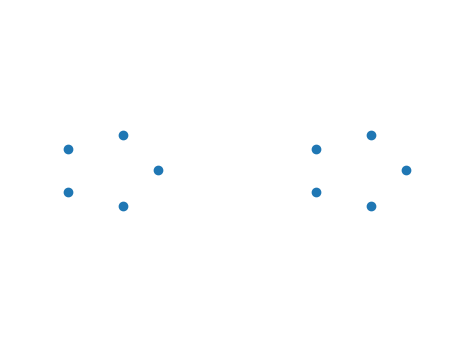
\includegraphics[width=\textwidth]{same_rotation.png}
  \caption{}\label{fig:same_rotation}
  \end{subfigure}
  \begin{subfigure}{0.45\textwidth}
  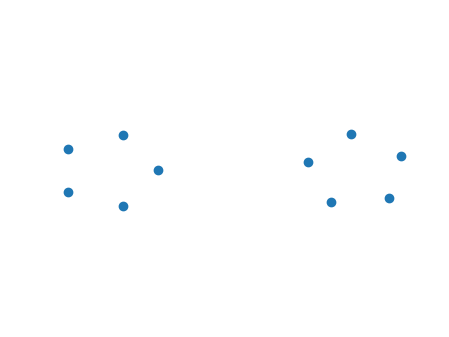
\includegraphics[width=\textwidth]{different_rotation.png}
  \caption{}\label{fig:different_rotation}
  \end{subfigure}
  \caption{A top-down (xy) view of the pore columns. (a) The right pore is an
  exact duplicate of the left including rotation about the z-axis. (b) The right
  pore is a duplicate of the left pore but rotated a random amount about the 
  z-axis.}\label{fig:initial_rotations}
  \end{figure}

  For a perfect, infinite crystal, the intensity of R-$\pi$ is infinitely sharp. We
  created a model with perfectly aligned columns. Each columns originates at z=0
  and all other points in the column are equally spaced 3.7 \AA~apart in the
  z-direction (Figure~\ref{fig:perfect_crystal_xyz}). This essentially creates
  layers of atoms. The intensity of R-$\pi$ for systems of various size are shown
  in Table~\ref{table:perfect_size_dependence}. The intensity of R-$\pi$ is equal
  to the number of atoms in the unit cell. The intensity will approach infinity as
  the system size becomes infinitely large.  

  \begin{figure}[!htb]
  \centering
  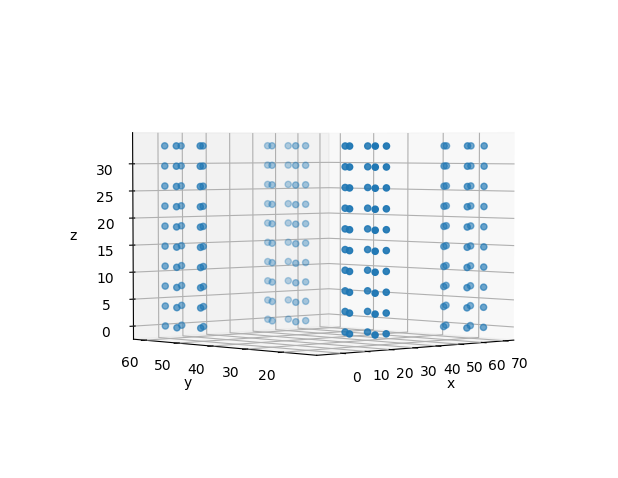
\includegraphics[width=0.5\textwidth]{perfect_crystal_xyz.png}
  \caption{}\label{fig:perfect_crystal_xyz}
  \end{figure}

  \begin{table}
  \centering
  \begin{tabular}{c c c c c}
  \toprule
  $L_z$ (\AA) & Points per column & Number of Pores &  Number of Atoms & R-$\pi$ Intensity\\ %& FWHM ($\AA^{-1}$) \\
  \midrule
  14.8        &      4            &       4          & 80               & 80              \\ %& 0.34  \\
  18.5        &      5            &       4          & 100              & 100             \\ %& 0.34  \\
  37          &      10           &       4          & 200              & 200             \\ %& 0.34  \\
  14.8        &      4            &       9          & 180              & 180             \\ %& 0.36  \\
  18.5        &      5            &       9          & 225              & 225             \\ %& 0.36  \\
  37          &      10           &       9          & 450              & 450             \\ %& 0.36  \\
  14.8        &      4            &       16         & 320              & 320             \\ %& 0.43  \\
  18.5        &      5            &       16         & 400              & 400             \\ %& 0.43  \\
  37          &      10           &       16         & 800              & 800             \\ %& 0.43  \\
  \bottomrule
  \end{tabular}
  \caption{The intensity of R-$\pi$ in a perfect crystal is equal to the number of
  scatterers in the unit cell. Here, $L_z$ is the length of the unit cell in the z direction which
  corresponds to number of points per column $\times$ 3.7.}\label{table:perfect_size_dependence}
  \end{table}

  We measured the peak width of R-$\pi$ in the $q_r$ direction using the
  appropriate slice of the structure factor. Ideally, one should use the angle
  averaged structure factor for this calculation, but since the angle averaging
  procedure interpolates between bins, the averaged intensities are lower than
  expected which slightly changes the shape of the peak and gives misleading
  results. This reflection is radially symmetric about the z-axis, so we fit peak
  widths to cross-sections at (0, y, 1.7)$^{-1}$ \AA (See Figure~\ref{fig:p2p_rpi}). 

  The distance between peaks in the $q_y$ cross-sections of the structure
  factor is equal to $2\pi / d$ (Figure~\ref{fig:p2p_rpi}), where d is the
  distance between pores. We looked at systems with pores spaced 42.5 nm and
  212.5 nm apart respectively. The fundamental frequency appears at $q_y=0$ with
  magnitude equal to the number of atoms in the unit cell (Note that each system
  has a different number of atoms). Subharmonics follow the fundamental frequency
  at equally spaced intervals of width $2\pi / d$. 

  \begin{figure}[!htb]
  \centering
  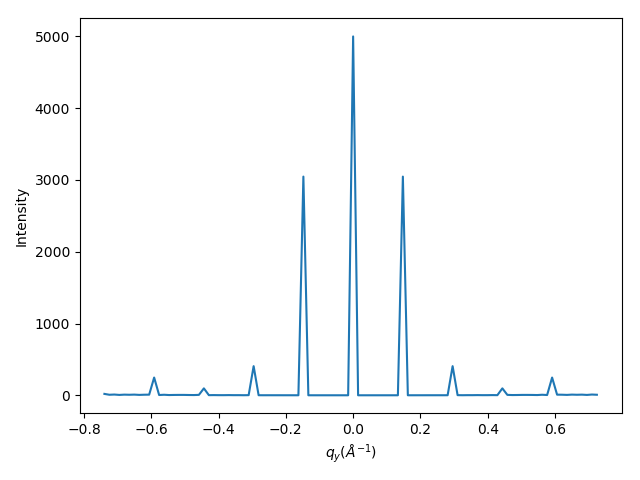
\includegraphics[width=0.45\textwidth]{constant_p2p.png}
  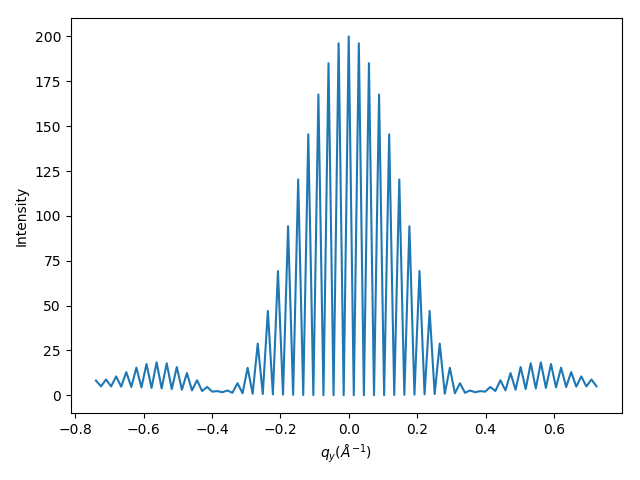
\includegraphics[width=0.45\textwidth]{constant_npores.png}
  \caption{The distance between peaks of the structure factor cross-section at
  (0, y, 1.7) is equal to the distance between pores in q-space. The center 
  peak of each distribution shows the fundamental frequency. The peaks
  that follow at higher $\left|\mathbf{q}\right|$ values are subharmonics. Both systems
  shown are in unit cells with dimensions of 42.5 x 42.5 x 3.7 nm. (a) We held
  the pore-to-pore spacing constant at 42.5 \AA. The unit cell consists of 100
  total pores. The first peak off-center peak is located at $q_y = .148 \AA^{-1}$
  which corresponds to $2\pi / .148 = 42.5 \AA$ in real space. (b) We placed four
  pores in a unit cell spaced 212.5 \AA~apart. The first peak appears where
  expected at $q_y = 0.0296 \AA^{-1}$ ($2\pi / 212.5 \AA$) and all other peaks
  are separated by that same distance.
  }\label{fig:p2p_rpi}
  \end{figure}

  We fit curves to the peaks of the cross-section of $q_y$ and measurd their
  full width at half maximum (FWHM). Gaussian profiles appear to give the closest
  fit to the data (see Figure~\ref{fig:fwhm_fits}). We calculated all of FWHMs in
  Table~\ref{table:perfect_size_dependence} using gaussian fits.

  \textbf{IMPORTANT}: Note that the FWHM does not translate to the peak widths
  that are seen experimentally. Rather it is a measure of the decay in the
  intensity of the off center peaks. Experimentally, the center peak is the only
  peak that appears and it is broadened. If the peaks here showed up
  experimentally, they would appear as dots parallel to the $q_r$ axis, crossing
  through R-$\pi$ and in line with R-pores. There is some evidence of this
  occuring in some of the simulations (ordered parallel displaced for example).

  \begin{figure}[!htb]
  \centering
  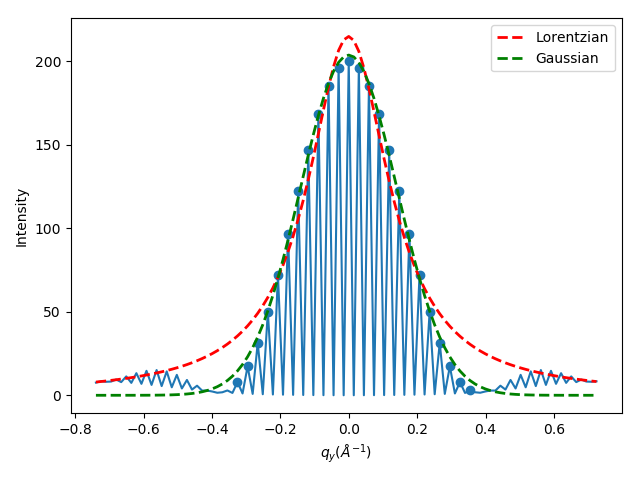
\includegraphics[width=0.5\textwidth]{fwhm_fits.png}
  \caption{The gaussian functional form more closely matches the data than the Lorentzian
  functional form. Shown is data for a perfect crystal system with 4 pores and 4 points
  per column.}\label{fig:fwhm_fits}
  \end{figure}

  The distance between pores does not affect the FWHM of the R-$\pi$ 'peak' in
  the $q_y$ direction.  We held the size of the unit cell constant at 42.5 x 42.5
  x 3.7 nm and varied the number of pores (and consequently, the distance between
  pores). We generated error bars for the fits based on the covariance of the
  optimized fit parameters. There is no statistical difference between the
  calculated values of each FWHM (Table~\ref{table:randomly_displaced_columns}).
  The uncertainty is lower for systems with less pores since there are more
  peaks available for curve fitting. 

  \begin{table}[!htb]
  \centering
  \begin{tabular}{c c c c c}
  \toprule
  $L_z$ (\AA) & Number of Pores & Distance between Pores &  R-$\pi$ intensity & FWHM ($\AA^{-1}$) \\
  \midrule
  37          &      4            & 212.5                & 200                & 0.372 $\pm$ 0.004 \\ 
  37          &      25           & 85.0                 & 1250               & 0.371 $\pm$ 0.008 \\
  37          &      100          & 42.50                & 5000               & 0.375 $\pm$ 0.013 \\
  \bottomrule
  \end{tabular}
  \caption{We held the size of the unit cell constant at 42.5 x 42.5 x 3.7 nm and varied the
   number of pores and distance between pores. The value of FWHM is indistinguishable between
   the systems.}\label{table:randomly_displaced_columns}
  \end{table}

  The finite FWHM of perfectly crystalline systems is due to non-uniform
  ordering of the columns within the pores. Although all scatterers are aligned
  and equally spaced in the z-direction, the individual columns of scatterers are
  offset from the pore center. Therefore, there is a range of similar but
  different distances between scatter scatterers. There are many opportunities
  for constructive and destructive interference with wavelengths slightly
  different than those which contribute to the fundamental frequency. If we place
  only one column at each pore center, the FWHM becomes infinite (See
  Figure~\ref{fig:infinite_FWHM})

  \begin{figure}[!htb]
  \centering
  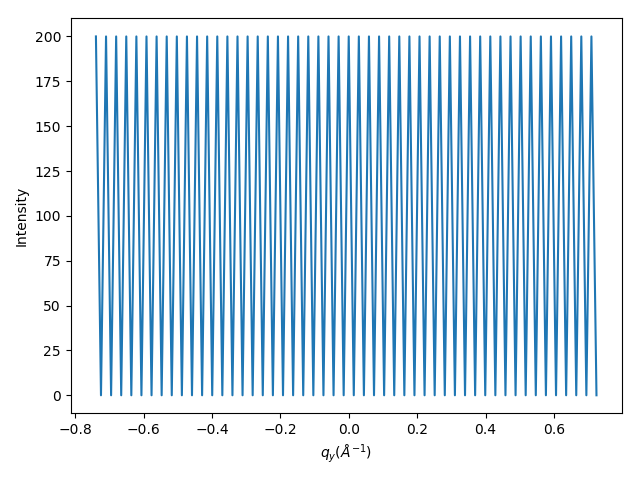
\includegraphics[width=0.5\textwidth]{one_column_per_pore.png}
  \caption{We placed one column of scatterers at each of 4 pore centers, spaced apart by
  212.5 nm. Since the y-component of the distance between all scatterers is the same in 
  all cases, subharmonics appear just as strongly as the fundamental frequency. Since the 
  intensity doesn't decay, the FWHM is infinite.}\label{fig:infinite_FWHM}
  \end{figure}

  The real system is far from a perfect crystal. In the proceeding section, we
  explore the influence of 4 sources of disorder on the intensity of R-$\pi$:
  \begin{enumerate}
  \item Random z-displacement of columns with respect to all other columns
  \item Random rotation of layers about the z-axis
  \item Thermal noise
  \item Finite correlation between scatterers in the z-direction
  \end{enumerate}

  \subsection{Imperfectly aligned columns}

  We randomly aligned columns along the z-axis by adding a random displacement
  to each column of points. This simulates a system in which columns are
  uncorrelated.  We wrapped coordinates where necessary so that all atoms stayed
  within the unit cell. We held the spacing between each point within each column
  at 3.7 \AA. We created trajectories of 1000 independent
  configurations in order to calculate the average intensity of R-$\pi$. 1000
  independent configurations gives a reasonably converged average, enough to
  observe trends.
 
  \textbf{NEW} We varied the degree to which we shifted each column with
  respect to other columns. The most we allowed the columns to shift was one full
  layer. To choose the position of the column, we chose a random displacement
  between 0 and d, where d is the maximum allowed displacement. We varied d
  between 0 and 3.7 \AA.  

  When d = 3.7 \AA, meaning columns are completely uncorrelated, the intensity
  of R-$\pi$ is equal to the number of scatterers per column (See
  Table~\ref{table:randomly_displaced_columns}).  It is independent of the number
  of pores (and hence number of columns) in the system. The error in the
  calculated intensities are comparable to the magnitude of the intensity because
  the intensity of each configuration in the trajectory fluctuates so much. 

  \begin{table}[!htb]
  \centering
  \begin{tabular}{c c c c c}
  \toprule
  $L_z$ (\AA) & Points per column & Number of Pores &  R-$\pi$ Intensity\\ 
  \midrule
  14.8        &      4            & 4               & 3.98              \\
  18.5        &      5            & 4               & 5.05              \\
  37          &      10           & 4               & 10.08             \\
  14.8        &      4            & 9               & 4.06              \\
  18.5        &      5            & 9               & 4.78              \\
  37          &      10           & 9               & 10.19             \\
  14.8        &      4            & 16              & 4.01              \\
  18.5        &      5            & 16              & 4.95              \\
  37          &      10           & 16              & 9.61              \\
  \bottomrule
  \end{tabular}
  \caption{The intensity of R-$\pi$ is equal to the number of scatters in each
	  column when columns are uncorrelated. Note that reproducing these results
	  requires a very fine histogram, and thus a much more expensive calculation. The
	  default binning scheme (100 bins in each dimension) gives slightly misleading
	  answers.
   }\label{table:randomly_displaced_columns}
  \end{table}

  \textbf{NEW} As we allow the columns to displace less (lower values of d),
  the intensity of R-$\pi$ increases (See Figure~\ref{fig:column_displacement}).
  Once there is no displacement, the intensity of R-$\pi$ matches that of a
  perfect crystal. The intensity of R-$\pi$ in the simulated system is likely
  boosted by the built-in correlation between columns.

  \begin{figure}[!htb]
  \centering
  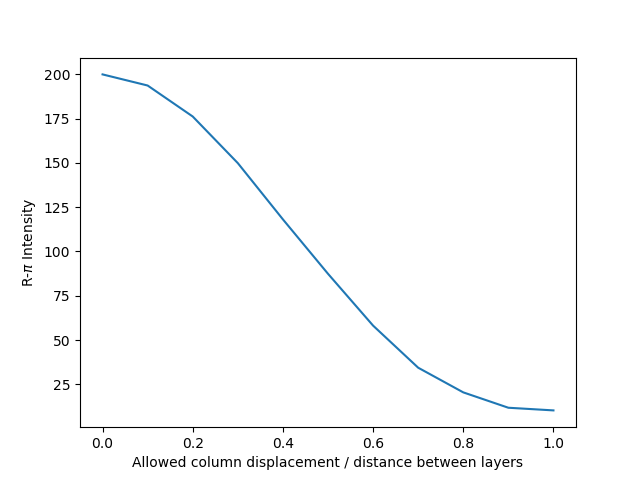
\includegraphics[width=0.5\textwidth]{column_displacement.png}
  \caption{As we increase the amount that columns are allowed to displace relative
  to each other, the intensity of R-$\pi$ decreases.}\label{fig:column_displacement}
  \end{figure} 

  The $q_y$ width of R-$\pi$ is infinite when columns are randomly displaced in
  the z-direction. We attempted to measure the FWHM of the system with randomly
  displaced columns containing 4 pores and $L_z = 37$. The cross-section
  (Figure~\ref{fig:random_columns_qy}) shows non-decaying noise centered near 10,
  the same R-$\pi$ intensity measured and shown in
  Table~\ref{table:randomly_displaced_columns}. The angle averaged pattern
  (Figure~\ref{fig:random_columns_rzplot}) further illustrates the diffraction
  lines which characterize this type of system.

  \begin{figure}[!htb]
  \centering
  \begin{subfigure}{0.45\textwidth}
  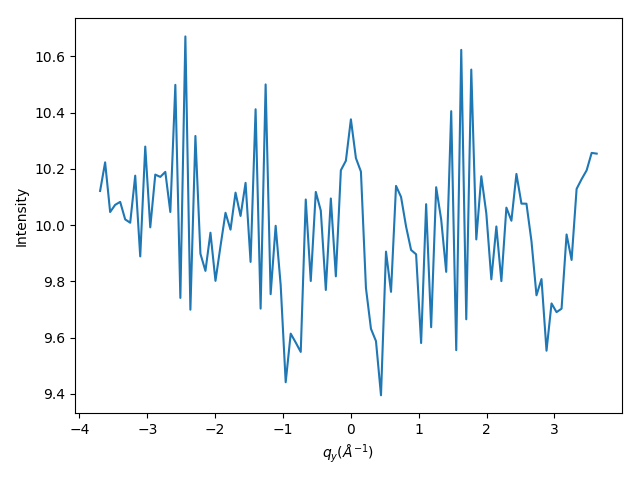
\includegraphics[width=\textwidth]{random_columns_qy.png}
  \caption{}\label{fig:random_columns_qy}
  \end{subfigure}
  \begin{subfigure}{0.45\textwidth}
  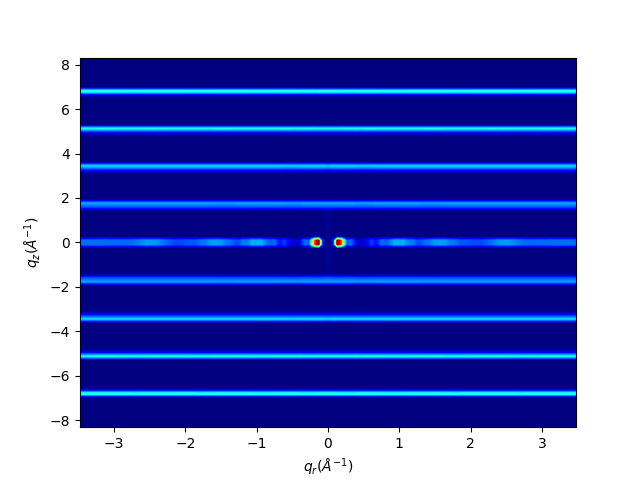
\includegraphics[width=\textwidth]{random_columns_rzplot.png}
  \caption{}\label{fig:random_columns_rzplot}
  \end{subfigure}
  \caption{When columns are uncorrelated, (a) the FWHM of the $q_y$
	  cross-section of the structure factor is infinite with a magnitude equal to the
	  number of scatterers per column. (b) The 2D structure factor angle averaged 
          about the z-axis shows diffraction lines spaced apart by 2$\pi$/d where d is the
          distance between scatterers in the z-direction.}\label{fig:random_columns_rpi_width}
  \end{figure}

  \subsection{Randomly rotated layers}

  We observed the influence of correlation between layers by randomly rotating layers
  of scatterers about the z-axis. We held constant the angle, with respect to the pore
  center, between scatterers for any given layer. For example, since there are 5 
  columns per pore, each layer is made of 5 monomers. The angle made between the two 
  vectors extending from the pore center to two adajacent scatterers in a single layer
  is 72 $\degree$ with respect to the xy plane.  

  \begin{table}[!htb]
  \centering
  \begin{tabular}{c c c c c c}
  \toprule
  $L_z$ (\AA) & Points per column & Number of Pores & Number of Atoms & R-$\pi$ Intensity & FWHM $\AA^{-1}$ \\
  \midrule
  14.8        &      4            & 4               & 80              &  80               & 0.37           \\
  18.5        &      5            & 4               & 100             &  100              & 0.37           \\
  37          &      10           & 4               & 200             &  200              & 0.37           \\
  14.8        &      4            & 9               & 180             &  180              & 0.37           \\
  18.5        &      5            & 9               & 225             &  225              & 0.37           \\
  37          &      10           & 9               & 450             &  450              & 0.37           \\
  14.8        &      4            & 16              & 320             &  320              & 0.37           \\
  18.5        &      5            & 16              & 400             &  400              & 0.37           \\
  37          &      10           & 16              & 800             &  800              & 0.37           \\
  \bottomrule
  \end{tabular}
  \caption{The intensity of R-$\pi$ is equal to the number of scatters in
   each column when columns are uncorrelated. Note that reproducing these results requires a very fine histogram, 
   and thus a much more expensive calculation. The default binning scheme (100 bins in each dimension) gives slightly
   misleading answers.}\label{table:randomly_rotated_layers}
  \end{table}

  In all cases, the maximum intensity of R-$\pi$ is equal to the number of
  scatterers in the system and the FWHM of the $q_y$ cross-section of the
  structure factor at R-$\pi$ is 0.37 $\AA^{-1}$
  (Figure~\ref{table:randomly_rotated_layers}), just as the perfect crystal.

  \textbf{NEW} There is no major difference in the intensity of R-$\pi$ between
  a perfect crystal and a system with randomly rotated layers. In the z
  direction, R-$\pi$ remains constant since the z components of the points are
  spaced exactly 3.7 \AA~apart. The maximum intensity of R-$\pi$ is at ($q_x,
  q_y, q_z$) = (0, 0, 1.7) so there is no contribution from the x or y
  components. Figure~\ref{fig:perfect_v_random_layers} shows a comparison of the
  cross-section of R-$\pi$ along $q_y=0$. On the surface it appears that there is
  a difference between them at high values of $q_y$. However, this is dependent
  on the initial configuration of the perfect crystal system. The system with
  randomly rotated layers will always look as it does if a sufficient number of
  configurations are included in the calculation of the structure factor. The
  perfect system is in agreement with the randomly rotated layer system at low
  values of $q_y$, corresponding to scatterers spaced far apart, however it begins
  to deviate at large $q_y$, where it describes the spatial relationship between
  scatterers in a single pore. In the perfect system, pores are randomly rotated
  with respect to each other (See Figure~\ref{fig:same_rotation}), so the spatial
  relationship changes each time a system is set up. It will not average out since
  each frame is exactly the same, but if enough pores are added, the 2 
  cross-sections will match (See Figure~\ref{fig:perfect_v_random_100pores}). 
  If we create a perfect crystal system where pores are duplicated and translated, but
  not rotated (See Figure~\ref{fig:same_rotation}), the subharmonics
  at large $q_y$ are quite pronounced (Figure~\ref{fig:perfect_crystal_same_rotation})
  due to the increase in ordering in the $q_y$ direction. The peaks are likely
  geometrically related to the spacing between points within pores, but it is 
  not important to get to the bottom of that here.

  \begin{figure}[!htb]
  \centering
  \begin{subfigure}{0.3\textwidth}
  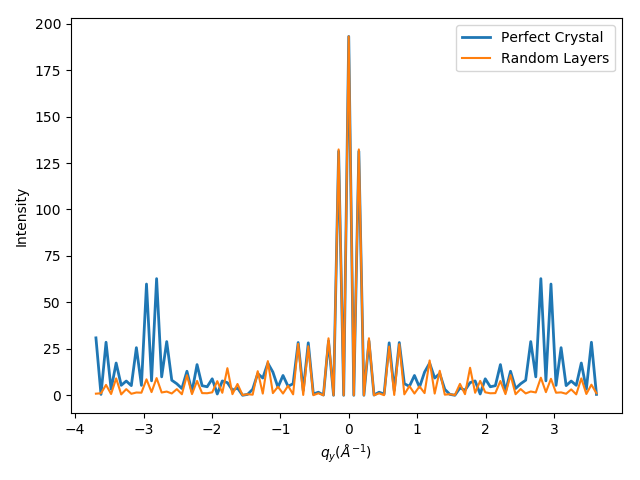
\includegraphics[width=\textwidth]{perfect_v_random_layers.png} 
  \caption{}\label{fig:perfect_v_random_layers}
  \end{subfigure}
  \begin{subfigure}{0.3\textwidth}
  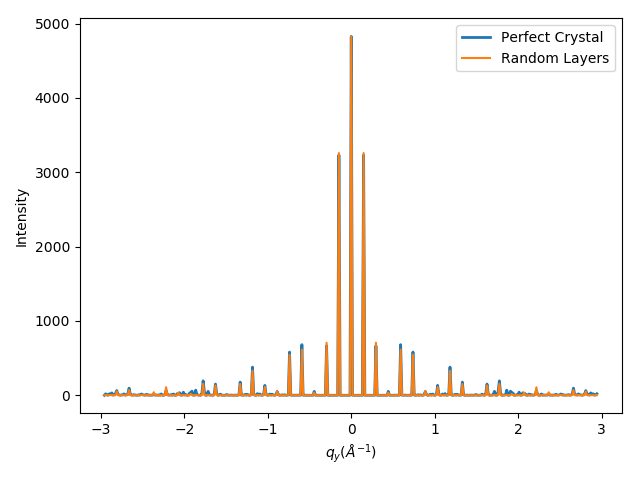
\includegraphics[width=\textwidth]{perfect_v_random_100pores.png} 
  \caption{}\label{fig:perfect_v_random_100pores}
  \end{subfigure}
  \begin{subfigure}{0.3\textwidth}
  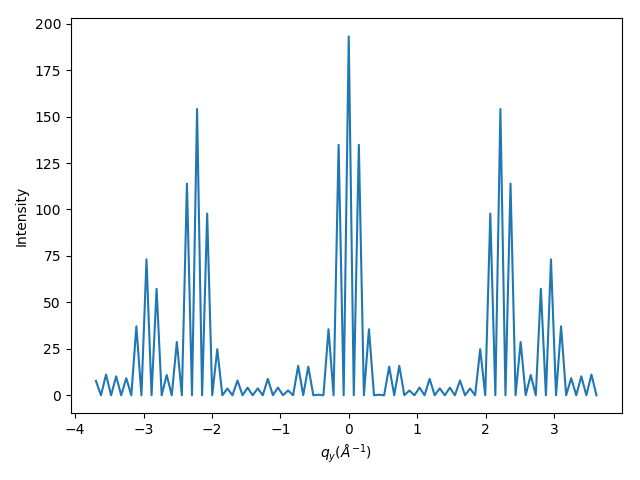
\includegraphics[width=\textwidth]{perfect_crystal_same_rotation_qy.png} 
  \caption{}\label{fig:perfect_crystal_same_rotation}
  \end{subfigure}
  \caption{\textbf{NEW} Shown are cross-sections of the 3D structure factor
  along $q_y$ at the $q_z$ value of R-$\pi$. We compare the cross-section for 
  a perfect crystal system and a system where layers are randomly rotated with
  respect to vertically adjacent layers. (a) When systems are made with 4 pores,
  the cross-sections agree at low $q_y$ values, however they diverge at higher
  values of $q_y$. (b) When we build the systems with 100 pores, the cross-sections
  are in close agreement. (c) If we do not rotate the pores in the perfect crystal
  system, there are large spikes at high values of $q_y$ due to order within pores.}\label{fig:perfect_v_layers}
  \end{figure}


%  \subsection{Influence of Pore Radius}

%  The pore radius is inversely proportional to the FWHM of systems made with
%  randomly rotated layers (See Figure~\ref{fig:pore_radius}). This result is not
%  extremely surprsing, although the limits of the relationship suggest that a
%  pore radius of 0 should give an infinite FWHM (supported by Figure
%  ~\ref{fig:infinite_FWHM}) and an infinitely large pore radius should have a
%  zero FWHM (of course the pore radius is limited by proximity to other pores).

%  This result is also interesting because it suggests that one can measure
%  relative pore radii using X-ray diffraction. The difficulty, which is
%  associated with the phase problem, is deconvoluting the electron density
%  associated with just pore entities.  
  
%  Since the maximum intensity of R-$\pi$ in a randomly rotated layer system
%  does not change with pore radius (it only depends on the total number of
%  scatterers), the FWHM is really just a measure of the decay of the subharmonics
%  surrounding $q_y=0$.

%  \begin{figure}[!htb]
%  \centering
%  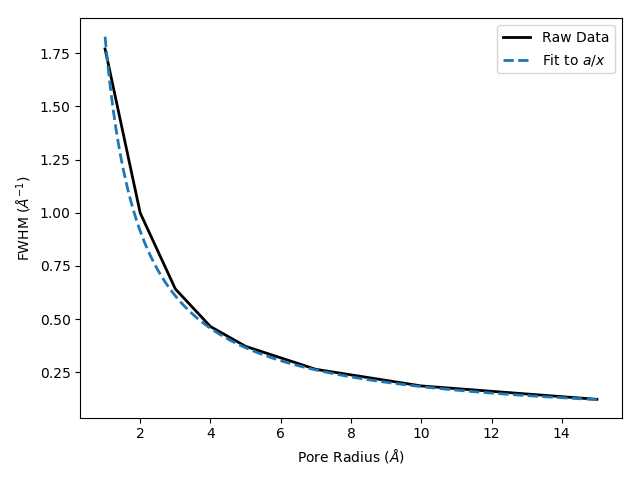
\includegraphics[width=0.5\textwidth]{pore_radius_FWHM.png}
%  \caption{The FWHM decays with increasing pore radius.}\label{fig:pore_radius}
%  \end{figure}

%  \begin{table}
%  \centering
%  \begin{tabular}{c c c c c c}
%  \toprule
%  $L_z$ (\AA) &   Pore Radius ($\AA^{-1}$) & FWHM ($\AA^{-1}$)  \\
%  \midrule
%  37          &      1                     &     1.770          \\
%  37          &      2                     &     0.999          \\
%  37          &      3                     &     0.642          \\
%  37          &      4                     &     0.465          \\
%  37          &      5                     &     0.372          \\
%  37          &      7	                   &     0.264          \\
%  37          &      10                    &     0.186          \\
%  37          &      15                    &     0.123          \\
%  \bottomrule
%  \end{tabular}
%  \caption{All systems contain four pores with 5 columns per pore and a unit cell
%  size of 42.5x42.5x3.7 nm. 
%  }\label{table:pore_radius}
%  \end{table}

  \subsection{The influence of thermal disorder}

  We added gaussian noise in each dimension to observe its influence on the
  intensity of R-$\pi$ and the FWHM. For the z-direction, the standard deviation
  of the gaussian distribution is equal to a fraction of the average distance
  between scatterers in columns (d). In the xy-directions, the standard deviation
  is equal to a fraction of the pore radius (r).

  \subsubsection{\textbf{NEW} Perfect Crystal}

  When we add z-direction gaussian noise to the lattice sites in the perfect
  crystal, the intensity of R-$\pi$ drops precipitously as noise is increased
  (Figure~\ref{fig:z_noise_perfect}).  However, the FWHM in the $q_y$ direction
  is unaffected by this noise (not pictured).

  When we add gaussian noise in the x and y directions, the intensity of
  R-$\pi$ does not change, however the FWHM sharpens with increasing noise
  (Figure~\ref{fig:xy_noise_perfect}). In other words, the intensity of
  subharmonics decrease, resulting in a smaller FWHM.  

  \begin{figure}[!htb]
  \centering
  \begin{subfigure}{0.45\textwidth}
  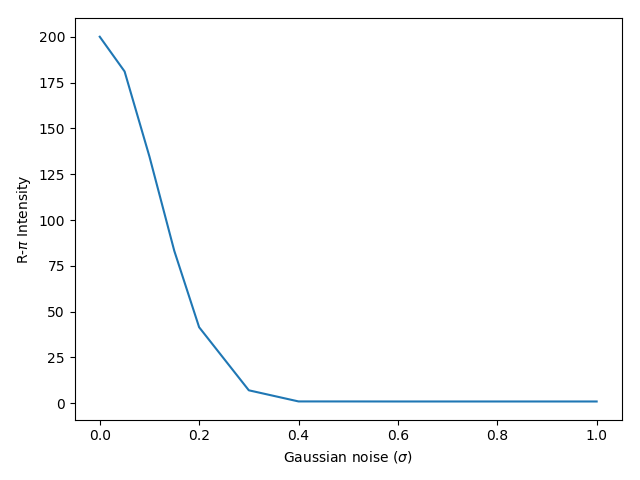
\includegraphics[width=\textwidth]{z_noise_perfect.png}
  \caption{}\label{fig:z_noise_perfect}
  \end{subfigure}
  \begin{subfigure}{0.45\textwidth}
  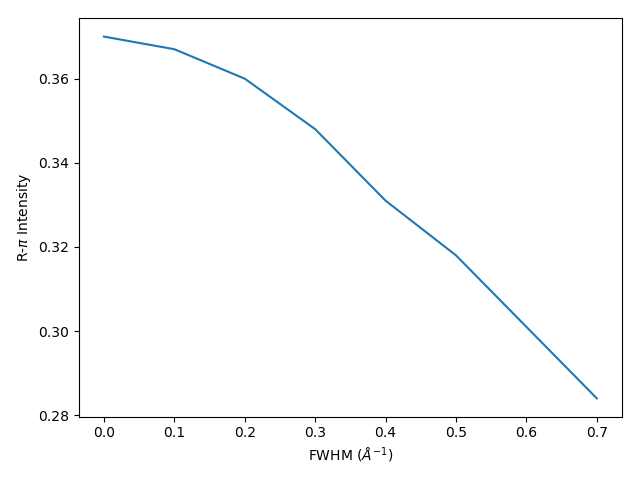
\includegraphics[width=\textwidth]{xy_noise_perfect.png}
  \caption{}\label{fig:xy_noise_perfect}
  \end{subfigure}
  \caption{(a) The intensity of R-$\pi$ decreases as the amount of z-direction
  noise increases. (b) The FWHM decreases as noise in the x and y directions
  increases.}\label{fig:perfect_noise}
  \end{figure}

  \subsubsection{Randomly displaced columns}

  When we add noise in the z direction, the intensity of R-$\pi$ decays
  (Figure~\ref{fig:z_noise_columns}).

  When we add noise in the x and y directions, R-$\pi$ has a finite peak width
  in its $q_y$ dimension (Figure~\ref{fig:FWHM_fit_columns}), and the intensity
  stays constant. This is different than what was previously shown
  (Figure~\ref{fig:fwhm_fits} for example). These are continuous peaks that
  represent broadening of the fundamental R-$\pi$ peak. We fit a Gaussian
  function to the the $q_y$ cross-section in order to determine its FWHM. The
  FWHM decay is inversely proportional to the amount of noise added
  (Figure~\ref{fig:FWHM_columns}). 

  \begin{figure}[!htb]
  \centering
  \begin{subfigure}{0.32\textwidth}
  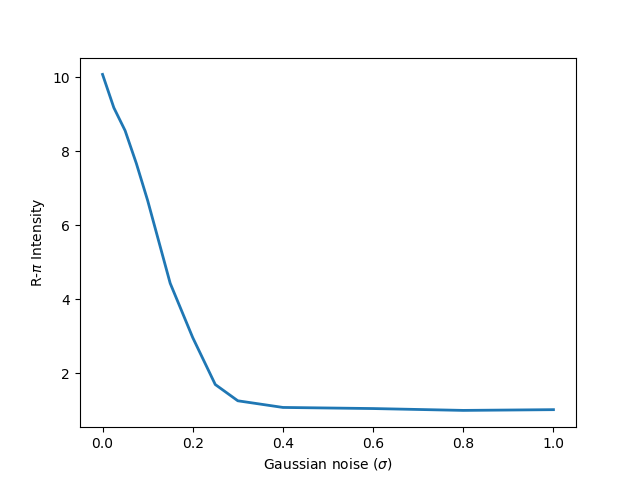
\includegraphics[width=\textwidth]{random_columns_z_noise.png}
  \caption{}\label{fig:z_noise_columns}
  \end{subfigure}
  \begin{subfigure}{0.32\textwidth}
  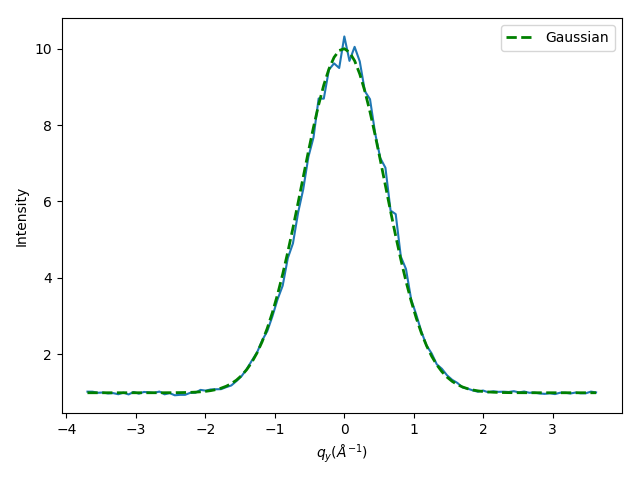
\includegraphics[width=\textwidth]{random_columns_gaussian.png}
  \caption{}\label{fig:FWHM_fit_columns}
  \end{subfigure}
  \begin{subfigure}{0.32\textwidth}
  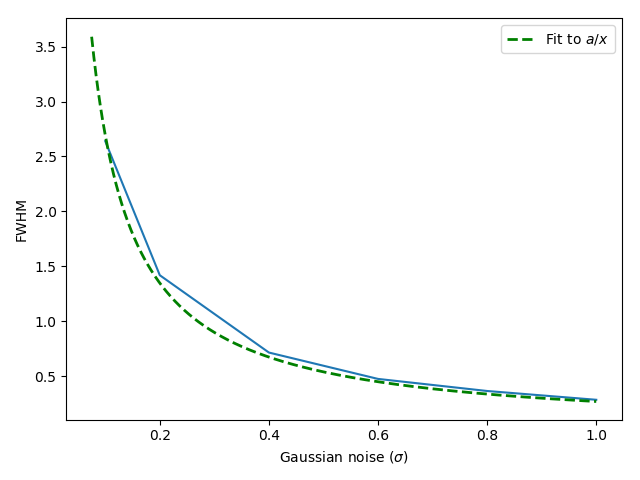
\includegraphics[width=\textwidth]{random_columns_xy_noise.png}
  \caption{}\label{fig:FWHM_columns}
  \end{subfigure}
  \caption{(a) The intensity of R-$\pi$ decays to 1 rapidly as gaussian noise is 
   added to the system. (b) When we add noise in the x and y directions, R-$\pi$
   broaden in the y-direction with a continuous intensity distribution that can be
   fit to a gaussian. (c) The FWHM decreases as the inverse of the amount of 
   noise added.}\label{fig:columns_noise}
  \end{figure}

  This mode of broadening of R-$\pi$ is more consistent with the experimental
  pattern, where the $q_y$ cross-section of R-$\pi$ is a continuous, broad peak. 

  \subsubsection{Randomly rotated layers}

  When we add noise in the z direction, the intensity of R-$\pi$ decays to 1
  rapidly (Figure~\ref{fig:random_layers_z_noise}), much like the decay shown in
  Figure ~\ref{fig:z_noise_columns}. The FWHM slowly increases until it jumps to
  infinity when the intensity of R-$\pi$ is comparable to the background
  intensity.

  When we add noise in the x and y directions, the intensity of R-$\pi$ does
  not change. The FWHM slowly decays as shown in
  Figure~\ref{fig:random_layers_xy_noise}. Importantly, the peak is defined by
  spikes like those shown in Figure~\ref{fig:p2p_rpi}.

  \begin{figure}
  \centering
  \begin{subfigure}{0.45\textwidth}
  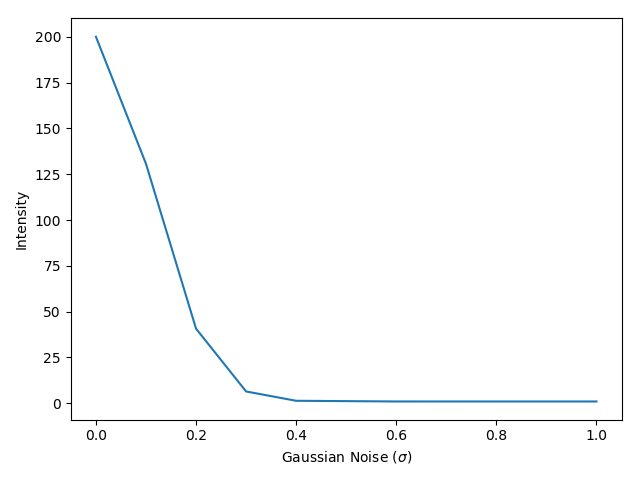
\includegraphics[width=\textwidth]{random_layers_z_noise.png}
  \caption{}\label{fig:random_layers_z_noise}
  \end{subfigure}
  \begin{subfigure}{0.45\textwidth}
  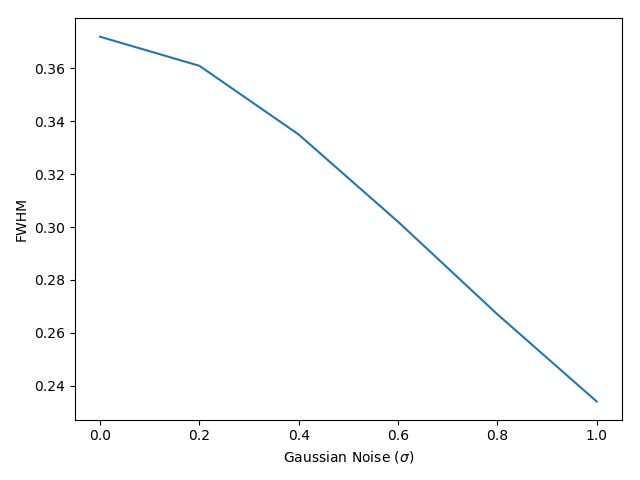
\includegraphics[width=\textwidth]{random_layers_xy_noise.png}
  \caption{}\label{fig:random_layers_xy_noise}
  \end{subfigure}
  \caption{(a) As we add noise in the z-direction, the intensity of R-$\pi$ decreases
   rapidly to 1. The FWHM increases slowly and then jumps to infinity (not pictured) 
   when the intensity of R-$\pi$ becomes equal to the background intensity. However one 
   could argue there is no peak at that point. (b) When we add noise in the x and y 
   directions, the intensity of R-$\pi$ does not change, but the FWHM decays slowly.}\label{fig:layers_noise}
  \end{figure}

  \subsubsection{Finite z-correlations}

  The z-cross-section of the R-$\pi$ peaks are delta functions in all of the
  above systems (See Figure~\ref{fig:deltas}). None of the routes explored so far
  show how R-$\pi$ might broaden in the $q_z$ direction. The delta-function
  behavior does not change when the system is made taller so as to increase the
  resolution in z. We built a system 10x taller (37 nm), added random column
  displacement and some noise in the z-direction. R-$\pi$ is still a sharp delta
  function (Figure~\ref{fig:tall_rpi}). 

  \begin{figure}
  \centering
  \begin{subfigure}{0.45\textwidth}
  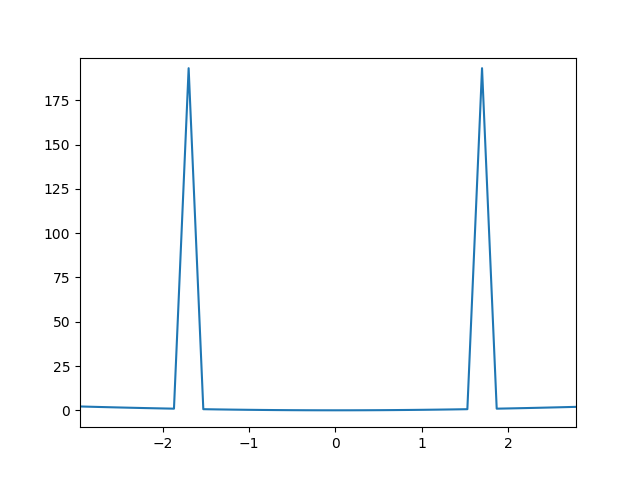
\includegraphics[width=\textwidth]{perfect_rpi.png}
  \caption{Perfect Crystal}\label{fig:perfect_rpi}
  \end{subfigure}
  \begin{subfigure}{0.45\textwidth}
  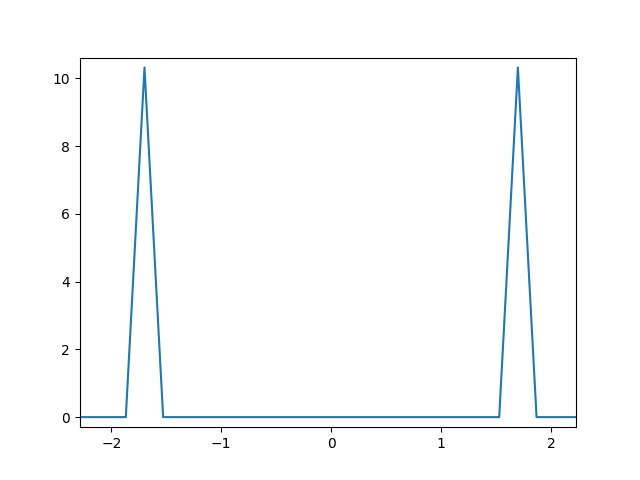
\includegraphics[width=\textwidth]{displace_columns_rpi.png}
  \caption{Randomly displaced columns}\label{fig:displaced_columns_rpi}
  \end{subfigure}
  \begin{subfigure}{0.45\textwidth}
  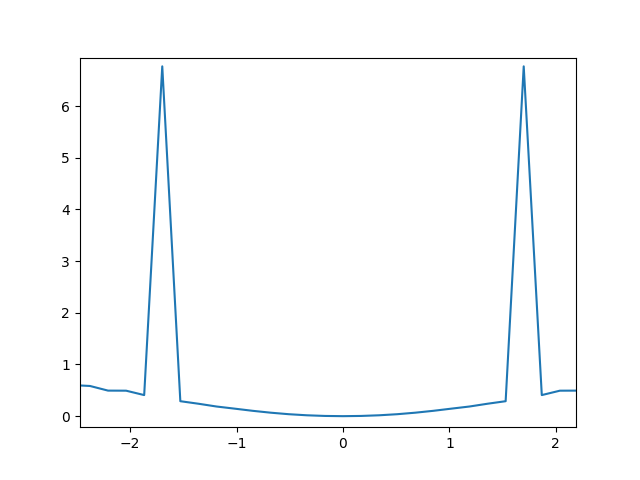
\includegraphics[width=\textwidth]{displaced_columns_z_noise_rpi.png}
  \caption{Randomly displaced columns w/ z-noise}\label{fig:displaced_columns_z_noise_rpi}
  \end{subfigure}
  \begin{subfigure}{0.45\textwidth}
  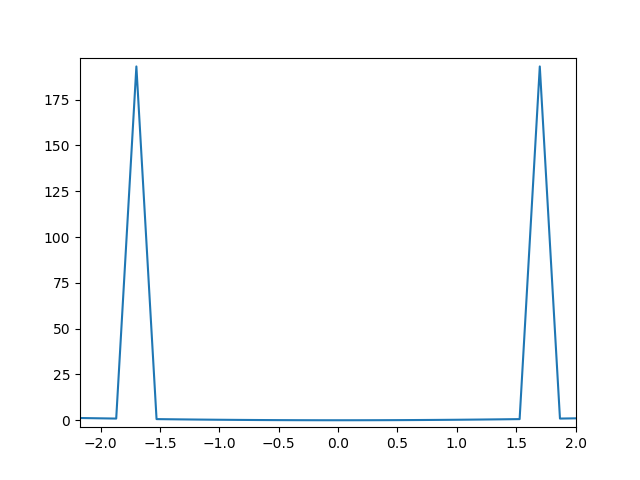
\includegraphics[width=\textwidth]{rotated_layers_rpi_xy_noise.png}
  \caption{Randomly rotated layers w/ xy-noise}\label{fig:rotated_layers_rpi_xy_noise}
  \end{subfigure}
  \caption{Several examples of the delta-like behavior of R-$\pi$. Randomly displacing
  columns, randomly rotating layers, and adding thermal disorder do not broaden 
  the z-cross-section of R-$\pi$.}\label{fig:deltas}
  \end{figure}

  \begin{figure}[!htb]
  \centering
  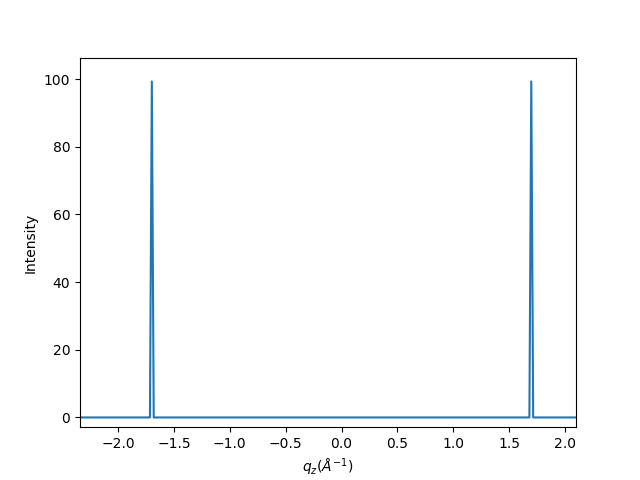
\includegraphics[width=0.5\textwidth]{tall_rpi.png}
  \caption{R-$\pi$ still appears to be a delta function even with higher resolution and
  noise in the z-positions of the scatterers}\label{fig:tall_rpi}
  \end{figure}

  (Please let me know if there is a more correct way of doing this)
  We added a correlation length to scatterers in z-direction. To do so, we
  define a covariance matrix to describe the correlation between all pairs of
  scatterers. The variance is defined so that the covariance in position of
  a scatterer with itself is the same for all scatterers. The covariance in
  position between scatterers decays exponentially from v according to the
  equation $ve^{-z/L}$ where L is the correlation length. Note that in its
  current implementation, it does not take periodicity into account, so a
  correlation length shorter than the box is necessary. A visualization of a
  typical covariance matrix for a column containing 20 scatterers is shown in
  Figure~\ref{fig:covariance}. Next, we drew random samples from a multivariate
  normal distribution defined using the covariance matrix, and applied these
  shifts to the columns of scatterers.

  \begin{figure}[!htb]
  \centering
  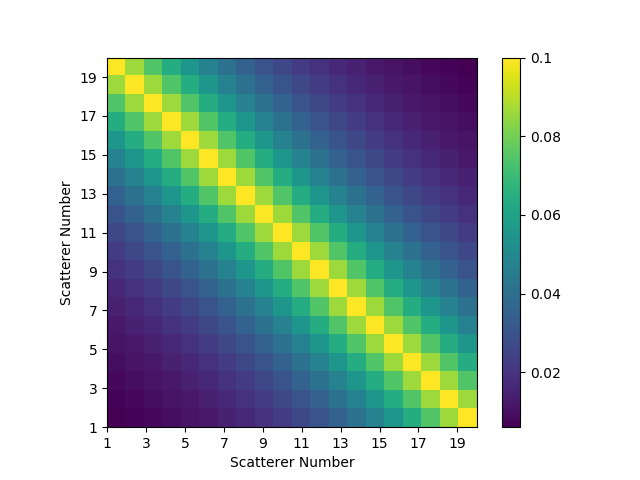
\includegraphics[width=0.5\textwidth]{covariance.png}
  \caption{An example covariance matrix used to place scatterers with a
	  correlation length. The scatterer centers are equally spaced in the
	  z-direction. Each value in the diagram represents the covariance between pairs
	  of scatterers. Diagonal entries represent covariance in position of scatterers
	  with themselves. The covariance decays exponentially as scatterers space apart
	  further.}\label{fig:covariance}
  \end{figure}

  Adding a finite correlation length between scatterers causes R-$\pi$ to
  broaden in the $q_z$ direction. We simulated a system with dimensions of 8.5 x
  8.5 x 37 nm, so that there would be 100 scatterers in the z-direction and a
  fourier bin size of $1/370=0.0027 \AA^{-1}$. There is a clear broadening of
  R-$\pi$ when scatterers are correlated
  (Figure~\ref{fig:correlation_comparison}). The maximum intensity of R-$\pi$
  decreases as the variance in scatterer position increases
  (Figure~\ref{fig:correlation_decay}), however the intensity of R-$\pi$ does not
  change when we vary the correlation length while holding the variance constant. 

  \begin{figure}[!htb]
  \centering
  \begin{subfigure}{0.45\textwidth}
  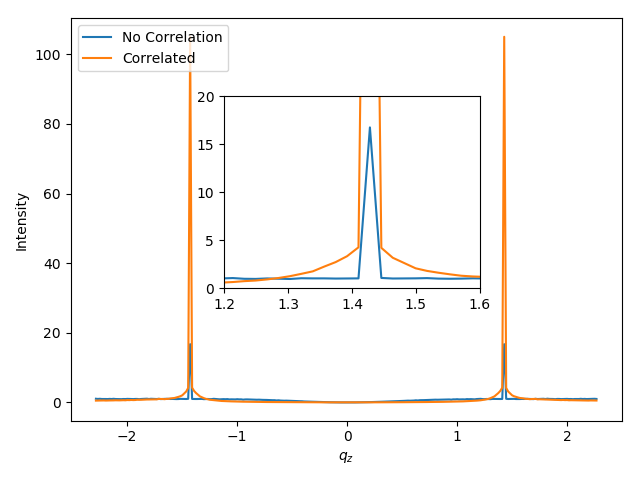
\includegraphics[width=\textwidth]{correlation.png}
  \caption{}\label{fig:correlation_comparison}
  \end{subfigure}
  \begin{subfigure}{0.45\textwidth}
  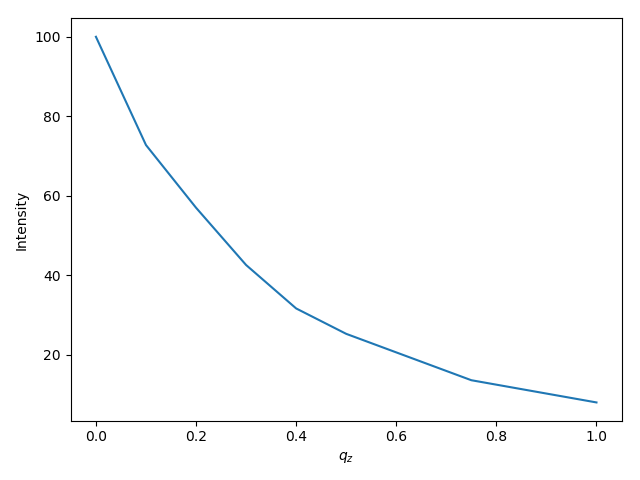
\includegraphics[width=\textwidth]{correlation_decay.png}
  \caption{}\label{fig:correlation_decay}
  \end{subfigure}
  \caption{(a) R-$\pi$ broadens in the $q_z$ direction when scatterers are
	  correlated. (b) The intensity of R-$\pi$ decreases as the variance in
	  scatterer position increases.}\label{fig:correlation}
  \end{figure}

  \subsubsection{\textbf{NEW} Systems with the "right" amount of noise}

  For a better understanding of the reasons why R-$\pi$ appears as it does in
  our simulated systems, we added a similar amount of noise to the model system
  as that seen in our simulations. Table ~\ref{table:simulation_noise} shows the
  amount of thermal noise in each dimension of the simulated system. We obtained
  those values by calculating the standard deviation in each dimension of the
  center of mass head group location from reference locations. We took the
  reference locations as the average center of mass of each head group. The
  standard deviations reported are only for frames over which we calculated the
  simulated diffraction patterns. 

  \begin{table}
  \centering
  \begin{tabular}{c c c c}
  \toprule
  System                         &   $\sigma_x$ ($\AA$) &   $\sigma_y$ ($\AA$) & $\sigma_z$ ($\AA$) \\
  \midrule
  Sandwiched, Ordered            &      0.31            &     0.33             &     0.34           \\
  Parallel Displaced, Ordered    &      0.51            &     0.52             &     0.30           \\
  Sandwiched, Disordered         &      0.41            &     0.57             &     0.32           \\
  Parallel Displaced, Disordered &      0.39            &     0.31             &     0.33           \\
  \bottomrule
  \end{tabular}
  \caption{Thermal noise in each dimension of the center of mass of monomer head groups for 
  simulated LLC systems}\label{table:simulation_noise}
  \end{table}

  Although the head groups do not move much in the equilibrated portion of the
  simulation, they are not arranged perfectly into columns. There is quenched
  disorder present from early in the simulation. To account for this noise, we
  measured the deviation of the center of masses from idealized positions. To
  calculate deviations in the x and y dimensions, we calculated the distance
  between each center of mass and the pore center. The distribution of the radial
  distance between each center of mass and the pore center, for the ordered
  sandwiched configuration, is shown in Figure~\ref{fig:xy_com_distribution}. To
  calculate deviations in the z dimension, we estimated the distance between
  layers to be the average z-box dimension divided by the number of scatterers
  per column (20 in the simulated system). Then we measured the deviation between
  the z position of each center of mass and its corresponding average z-layer
  position. Histograms of the deviations, for the ordered sandwiched
  configuration, are in Figure~\ref{fig:z_com_distribution}. We use the standard
  deviation of each distribution in Figure~\ref{fig:com_distribution} in order to
  place points in our model systems. The standard deviations for all systems
  are given in Table~\ref{table:com_sigmas}.  

  \begin{figure}[!htb]
  \centering
  \begin{subfigure}{0.45\textwidth}
  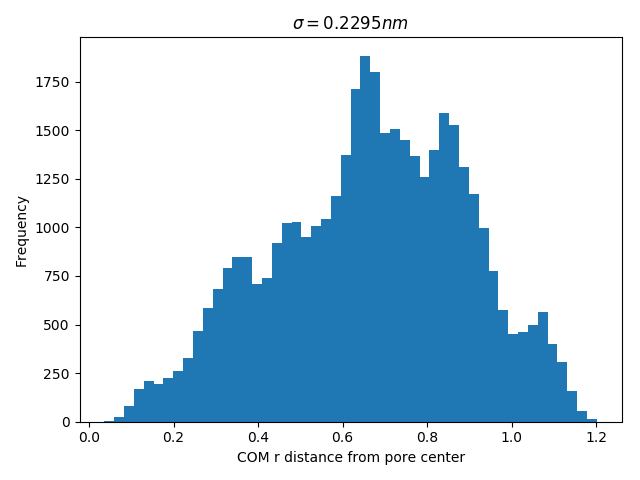
\includegraphics[width=\textwidth]{xy_com_distribution.png}
  \caption{}\label{fig:xy_com_distribution}
  \end{subfigure}
  \begin{subfigure}{0.45\textwidth}
  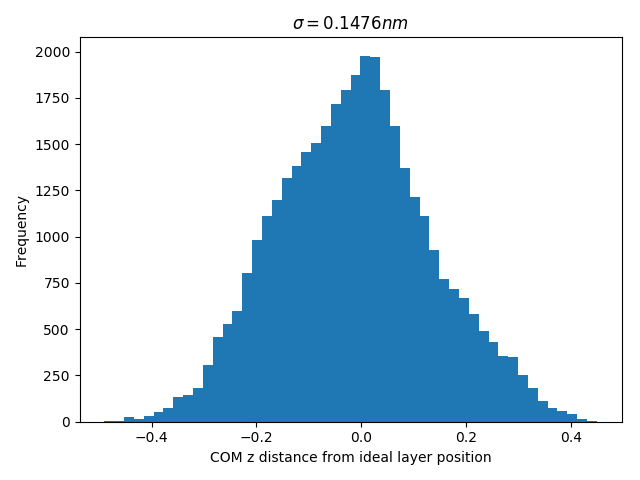
\includegraphics[width=\textwidth]{z_com_distribution.png}
  \caption{}\label{fig:z_com_distribution}
  \end{subfigure}
  \caption{}\label{fig:com_distribution}
  \end{figure}

  \begin{table}[!htb]
  \centering
  \begin{tabular}{c c c}
  \toprule
  System                         &   $\sigma_r$ ($\AA$) &   $\sigma_z$ ($\AA$) \\
  \midrule
  Sandwiched, Ordered            &      2.30            &     1.48             \\
  Parallel Displaced, Ordered    &      2.28            &     1.45             \\
  Sandwiched, Disordered         &      2.93            &     1.58             \\
  Parallel Displaced, Disordered &      2.63            &     1.65             \\
  \bottomrule
  \end{tabular}
  \caption{Uncertainty in the deviation of monomer head groups from ideal 
          positions in each dimension for simulated LLC systems}\label{table:com_sigmas}
  \end{table}

  For a good structural comparison, we set up a model system that mimics the
  ordered sandwiched configuration. We stacked scatterers 4.4 \AA apart and
  created pores with a radius of 6.6 \AA in order to be consistent with the
  values used to calculate the deviations in Table~\ref{table:com_sigmas}. We
  created an initial configuration with noise in the placement of points based on
  the values in Table~\ref{table:com_sigmas}. We made the scatterers correlated
  in the z-direction with a correlation length equal to 20 \AA which is about
  what we've measured in the simulations. Using the initial configuration, we
  created 1000 frames to which we added thermal noise in accordance with that
  measured and recorded in Table~\ref{table:simulation_noise}. The result is a
  center-of-mass trajectory that is configured and behaves similarly to the
  simulation trajectory. We can use that model to tune the various influences
  on R-$\pi$.

  The intensity of R-$\pi$ is strongly dependent on the initial configuration.
  Each time a model system is generated, the initial configuration is different
  than the previous model system. The thermal noise added does not compensate for
  these differences. We ran 40 different model systems with the only difference
  being the initial configuration randomization. The average R-$\pi$ intensity of
  the 40 trials was 25.7 $\pm$ 9.4. This spread has important implications for
  the reproducibility of our data since there is velocity randomization during
  the initial equilibration that will randomize the configurations which are 
  then locked in. Also, this initial configuration dependence is not
  very useful for analyzing trends. 

  We observe the same R-$\pi$ intensity when each frame of the trajectory is
  randomized. We created a trajectory of 1000 frames. We set up each frame as
  described in the paragraph before last, however with each frame independent. The
  average R-$\pi$ intensity over 1000 frames was 25.4, in close agreement with
  that calculated for the 40 trials of 100 dependent configurations in the
  previous paragraph. We can use this type of setup to analyze trends.  

  Allowing columns to displace further with respect to each other causes the
  intensity of R-$\pi$ to decrease (Figure~\ref{fig:ld}). In all of the above
  systems, we placed columns at exactly the same z displacement. Here we allowed
  them to displace from their initial centers as a function of the fraction of
  the distance between layers.

  Qualitatively, we can make R-$\pi$ look the most like experiment when columns
  move independently (See Figure~\ref{fig:rzplots}). As we decrease the
  dependence between columns, the intensity of R-$\pi$ decreases and the
  reflection spreads out in the $q_r$ direction. With any amount of dependence
  between columns, R-$\pi$ sharpens at the center of the reflection. 

  Again, R-$\pi$ decreases in response to thermal noise (See 
  Figure~\ref{fig:td}). We varied the amount of thermal noise from a 100 \%
  decrease to a 100 \% increase in noise in each dimension.

  An increased correlation length causes a modest, linear increase in the
  intensity of R-$\pi$ (Figure~\ref{fig:cl}). The effect is not nearly as
  pronounced as z-directional noise and column displacement.

  As we increase the amount of noise in the initial, quenched disordered
  configuration, the intensity of R-$\pi$ decreases (Figure~\ref{fig:IC}).  We
  changed the amount of order in the initial configuration by scaling the noise
  used during placement from -100 \% to 100 \%. We scaled noise in all three
  dimensions, however we know that the maximum intensity of R-$\pi$ will only be
  influenced by noise in the z direction.

  \begin{figure}
  \centering
  \begin{subfigure}{0.45\textwidth} 
  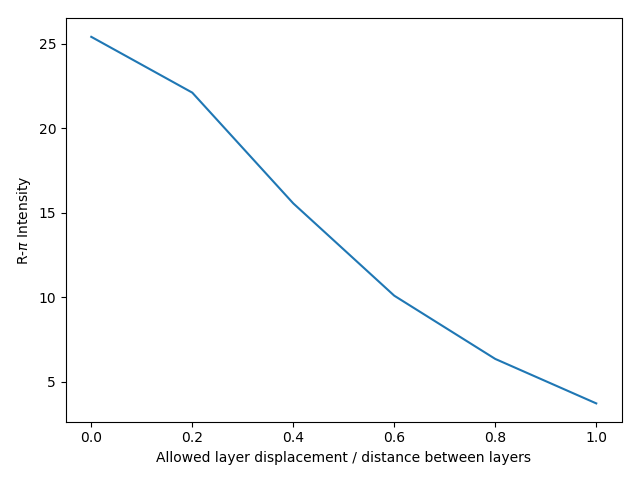
\includegraphics[width=\textwidth]{ld.png}
  \caption{}\label{fig:ld}
  \end{subfigure}
  \begin{subfigure}{0.45\textwidth} 
  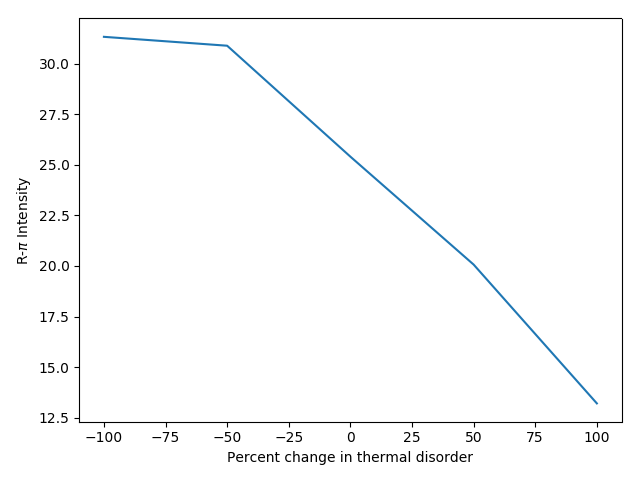
\includegraphics[width=\textwidth]{td.png}
  \caption{}\label{fig:td}
  \end{subfigure}
  \begin{subfigure}{0.45\textwidth} 
  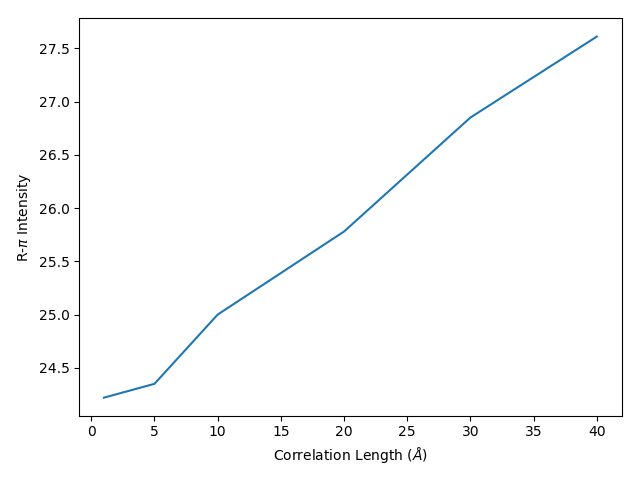
\includegraphics[width=\textwidth]{cl.png}
  \caption{}\label{fig:cl}
  \end{subfigure}
  \begin{subfigure}{0.45\textwidth} 
  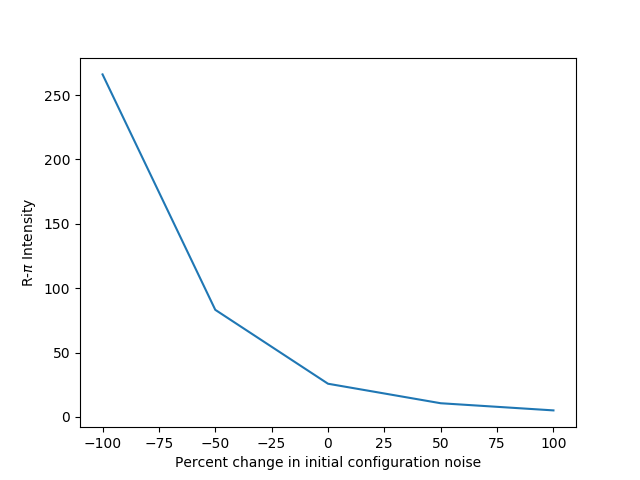
\includegraphics[width=\textwidth]{IC.png}
  \caption{}\label{fig:IC}
  \end{subfigure}
  \caption{(a) The intensity of R-$\pi$ decreases as the layers become more
  independent. (b) The intensity of R-$\pi$ decreases when thermal disorder
  decreases. (c) The intensity of R-$\pi$ increases with the correlation length.
  (d) The intensity of R-$\pi$ decreases as more noise is added to the initial
  configuration.}\label{fig:sim_comp}
  \end{figure}

  \begin{figure}
  \centering
  \begin{subfigure}{0.45\textwidth} 
  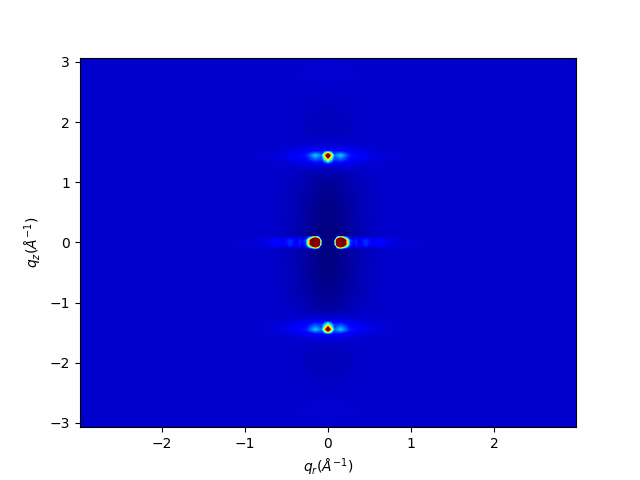
\includegraphics[width=\textwidth]{rzplot_ld0.png}
  \caption{}\label{fig:rzplot_ld0}
  \end{subfigure}
  \begin{subfigure}{0.45\textwidth} 
  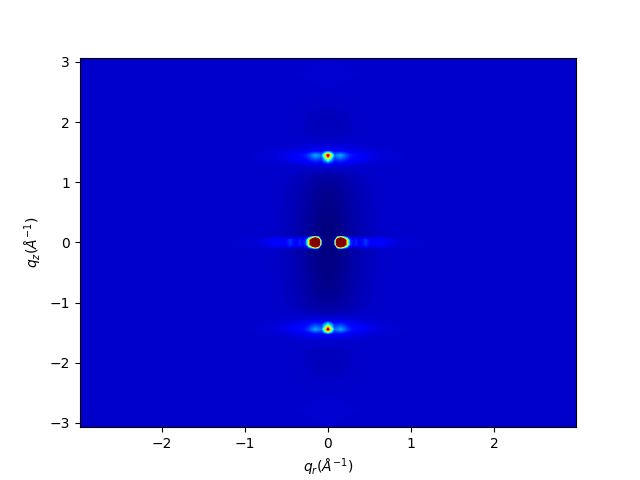
\includegraphics[width=\textwidth]{rzplot_ld33.png}
  \caption{}\label{fig:rzplot_ld33}
  \end{subfigure}
  \begin{subfigure}{0.45\textwidth} 
  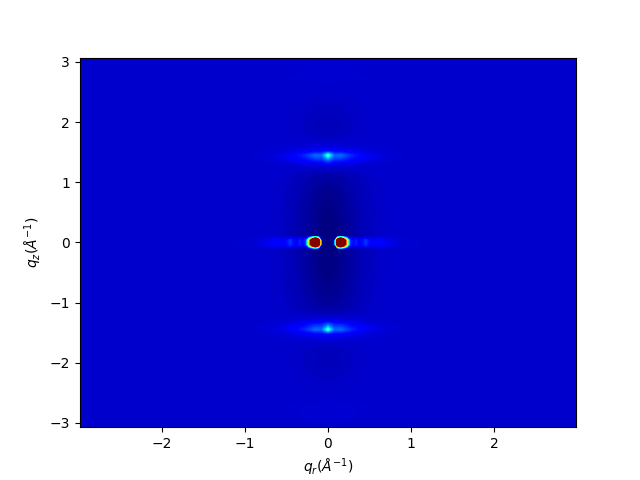
\includegraphics[width=\textwidth]{rzplot_ld66.png}
  \caption{}\label{fig:rzplot_ld66}
  \end{subfigure}
  \begin{subfigure}{0.45\textwidth} 
  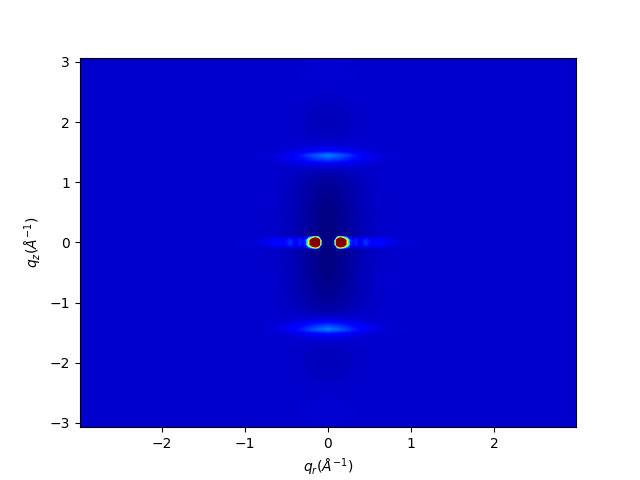
\includegraphics[width=\textwidth]{rzplot_ld1.png}
  \caption{}\label{fig:rzplot_ld1}
  \end{subfigure}
  \caption{As we allow layers to move more independently, the intensity of
  R-$\pi$ decreases and spreads out in the $q_r$ direction.}\label{fig:rzplots}
  \end{figure}


  \section{Conclusion}
 
  A number of factors influence the shape and intensity of the R-$\pi$ reflection
  in our simulated systems.
 
  The maximum intensity of the reflection is most strongly influenced by
  disorder in the z-direction. The first source of z-directional disorder is
  caused by randomization of the initial configuration.  This configuration gets
  essentially locked into place. The second source is thermal noise during the
  simulation. The amount of thermal noise is smaller in magnitude than the
  randomization induced during early equilibration. 

  The peak is broadened in the $q_y$ ($q_r$) direction when there is
  xy-direction thermal disorder in systems with randomly displaced columns. The
  peak looks most like experiment when columns are completely independent.
 
  The peak is broadened in the $q_z$ direction when there is a finite (non-zero)
  correlation length between scatterers.
 
\end{document}
